% deckblatt.tex, 2019/03/15 
\documentclass[a4paper,12pt]{article}  
%Inhaltsverzeichnis in Kapitel und Sektionen aufgeteilt  \chapter{title} > \section{title} > subsection{title} \subsubsection{title}

% Pakete und Paket-Configs
\usepackage{times} % Times Roman als Standardschrift
\usepackage[ngerman]{babel} % neue deutsche Rechtschreibung und Trennung
\usepackage{fancyhdr} % spezielle Kopfzeilen
\usepackage[latin1]{inputenc} % Umlaute ��� auch normal benutzen und nicht maskieren
\usepackage[babel, german=quotes]{csquotes}
\usepackage{subfigure} % Figures divided into subfigures.
\usepackage{ifthen} % Ermöglicht ifthenelse und whiledo
\usepackage{amsfonts} % Extra mathematical symbols
\usepackage[rflt]{floatflt} % verbessertes floatfig, als um figure's fliesende texte
\usepackage[T1]{fontenc} % ?? aber notwendig für korrekte PDF-Metadaten
%\usepackage{longtable} % Support for tables longer than a page.
%\usepackage{a4wide} % Increases width of printed area of an a4 page.
%\usepackage{alltt} % verbatim environment except that \ and braces have their usual meanings.
\usepackage{listings} % Typeset source code listings using LaTeX.
\usepackage{moreverb} % bessere verbatim-umgebungen
\usepackage{graphicx}
\usepackage{pdfpages}
\usepackage{caption}
\usepackage{xcolor} % Farben Definierbar \definecolor{fhorange}{RGB}{255,153,0}
\usepackage{biblatex} % F�r das Erstellen eines Literaturverzeichnisses
\addbibresource{literatur.bib}  % f�r das erstellen des Literaturverzeichnisses empfielt sich die Software Mendeley, diese erm�glicht einfaches hinzuf�gen B�chern und das exportieren in eine .bib Datei 
\usepackage{acronym}



\pagestyle{headings} % Kopf- und Fusszeilen
\pagenumbering{Roman} % Nummerierung der Seiten
\newcommand{\maximagewidth}{15cm} % maximal m�gliche Bildbreite

\setlength{\parindent}{0cm} % Einr�ckung am Abstzanfang
\setlength{\parskip}{5pt plus 2pt minus 1pt} % Abstand der Abs�tze zueinander
\frenchspacing % Kein Zusatzzwischenraum nach Satzzeichen

\setcounter{secnumdepth}{3} % Z�hlung bis paragraph 1.1.1
\setcounter{tocdepth}{3} % Inhaltsverzeichnis bis paragraph 1.1.1

%\makeglossary % Schreibe ein Glossar-File

\title{Titel der Arbeit}
\author{Name des Authors}
\date{\today}
\definecolor{fhorange}{RGB}{255,153,0}
\begin{document}
	
	\begin{titlepage}
		\thispagestyle{empty}
		\begin{center}
			\begin{minipage}{15cm}
				\begin{flushright}
					
\includegraphics[width=4cm]{fhlogo.png} \hspace{1.5cm} \\
					\textbf{\large Hochschule \hspace{3.5cm} ~ \\ Augsburg } \large University of \hspace{1cm} ~ \\ Applied Sciences \hspace{0.2cm} ~
					\\~
				\end{flushright}
				
				\begin{flushleft}
					\textbf{\large \textcolor{fhorange}{Hardwaresysteme\\K�rprojekt}} \hspace{8.35cm} \textcolor{fhorange}{\large Fakult�t f�r}
					\vspace{0.1cm}
					\\~  \hspace{10.75cm} \textcolor{fhorange}{\large Informatik} 
				\end{flushleft}
				
				%\vspace{1cm}
				\begin{flushleft}
					{ \large Studienrichtung \\ 
						%	\vspace{0.2cm}
						M.Sc. Informatik
					}
					\vspace{0.1cm}
				\end{flushleft}
				\begin{flushleft}
					{
						\textcolor{fhorange}{\large \textbf{Mathias Schoppe \\
								Entwicklung eines integrierten Schaltkreises - Konzeptionierung und Umsetzung}}
					}
					\vspace{0.2cm}
				\end{flushleft}
				\begin{flushleft}
					{ \large Betreuer: Prof. Dr.-Ing. Gundolf Kiefer \\ 
						\vspace{0.1cm}
						Abgabe der Arbeit am: 09.07.2023 			
					}
				\end{flushleft}
				\begin{flushleft}
					%In Kooperation mit Firma: \\ Hsa-Digit \\ Betreuer: Hans Mustermann \\ 
					%\vspace{0.5cm}
					%
\includegraphics[width=3cm]{hsa_digit.png} \hspace{5cm} 
					\tiny{\textcolor{gray}{
							\hspace{11.3cm} Hochschule f�r angewandte \\
							\hspace{11.3cm} Wissenschaften Augsburg \\
							\hspace{11.3cm} University of Applied Sciences \\ ~ \\
							\hspace{11.3cm} An der Hochschule 1 \\
							\hspace{11.3cm} D-86161 Augsburg \\ ~ \\
							\hspace{11.3cm} Telefon +49 821 55 86-0 \\
							\hspace{11.3cm} Fax +49 821 55 86-3222 \\
							\hspace{11.3cm} www.hs-augsburg.de \\
							\hspace{11.3cm} info@hs-augsburg.de \\} ~ \\
						\hspace{11.3cm} Fakult�t f�r Informatik \\
						\hspace{11.3cm} Telefon +49 821 5586-3450 \\
						\hspace{11.3cm} Fax ~~~ +49 821 5586-3499 \\ ~ \\
						\hspace{11.3cm} Verfasser der Ausarbeitung: \\
						\hspace{11.3cm} Mathias Schoppe \\
						\hspace{11.3cm} Matr. Nr.: 000000 \\
						\hspace{11.3cm} M. Sc. Informatik \\
						\hspace{11.3cm} Teamkollegen: Sascha Testname \\
						\hspace{11.3cm} und Timo Winklbauer \\
						
					}
				\end{flushleft}
			\end{minipage}
		\end{center}
	\end{titlepage}
	
	
	% Zusammenfassung
	\thispagestyle{empty}
	\section*{Abstract}
	\newpage
	\thispagestyle{empty}
	\tableofcontents  
	% Wenn das Inhaltsverzeichnis aktualisiert werden muss 2 mal kompilieren, erst dann wird die Aktualisierung angezeigt
	\newpage
	\pagenumbering{arabic}
	\section{Einleitung}
	\subsection{Motivation}
	In dieser Ausarbeitung liegt der Fokus auf der Entwicklung eines eigenen \acp{IC} mithilfe des Tiny-Tapeout-Projekts\cite{TT}. Der Prozess des \ac{IC}-Designs ist �u�erst komplex und erfordert spezialisierte Kenntnisse sowie teure Ausr�stung und Ressourcen. Das Tiny-Tapeout-Projekt hat es geschafft, ein besonderes Konzept zu entwickeln, das es selbst Anf�ngern erm�glicht, ihre eigenen \ac{IC}-Designs zu realisieren. Es bietet eine kosteng�nstige M�glichkeit, ein eigenen \ac{IC} fertigen zu lassen und er�ffnet somit neue M�glichkeiten f�r kreative Ideen und individuelle Schaltungen. Dieser Teil der Ausarbeitung behandelt Aspekte, welche f�r ein solches Vorhaben zu beachten sind und bezieht sich dabei auf die konkrete Umsetzung eines Reaktionsspiels als \ac{IC}.
	\subsection{Zielsetzung}
	Das Ziel der Arbeit besteht darin, ein eigenes \ac{IC}-Design f�r ein Reaktionsspiel zu entwerfen und zu simulieren. Hierbei wird darauf geachtet, dass maximal 500 Logikgatter und ausschlie�lich die Ein- und Ausg�nge des Tiny-Tapeout Evaluationsboards f�r die Umsetzung ben�tigt werden. Durch die Realisierung dieses Projekts sollen grundlegende Kenntnisse im IC-Design erlangt und praktische Erfahrungen in der Entwicklung von elektronischen Schaltungen gesammelt werden.
	\pagebreak
	\section{Grundlagen}
	Das nachfolgende Kapitel befasst sich mit grundlegenden Themen, welche f�r die Umsetzung der Arbeit unabdingbar sind. Die Themenbereiche werden zusammengefasst und so erl�utert, dass auch Lesende ohne Vorerfahrung im Bereich der Hardwareentwicklung alle Aspekte der Arbeit nachvollziehen k�nnen.
	\subsection{Linear r�ckgekoppeltes Schieberegister}
	Ein \acl{LFSR} (engl. linear feedback shift register (\acs{LFSR})) ist eine Schaltung, die aus einer Reihe von Flip-Flops (digitale Speicherelemente) besteht, die in einer Kette miteinander verbunden sind. Die R�ckkopplung erfolgt, indem das Ausgangssignal eines Flip-Flops mit dem Eingang eines vorherigen Flip-Flops verbunden wird. Dadurch bildet sich ein geschlossener R�ckkopplungs-Pfad. In Abbildung \ref{fig:lfsr} ist ein 8-Bit Fibonacci-\ac{LFSR} dargestellt. In der Abbildung stellt CLK den Takteingang und Y den Ausgang des \ac{LFSR} dar. Das Fibonacci-\ac{LFSR} zeichnet sich durch das primitive Generatorpolynom (formel: $$pf(x) = x^8 + x^6 + x^5 + x^4 + 1)$$ aus.
	\vspace{1em}
	
	\begin{minipage}{\linewidth}
		\centering
		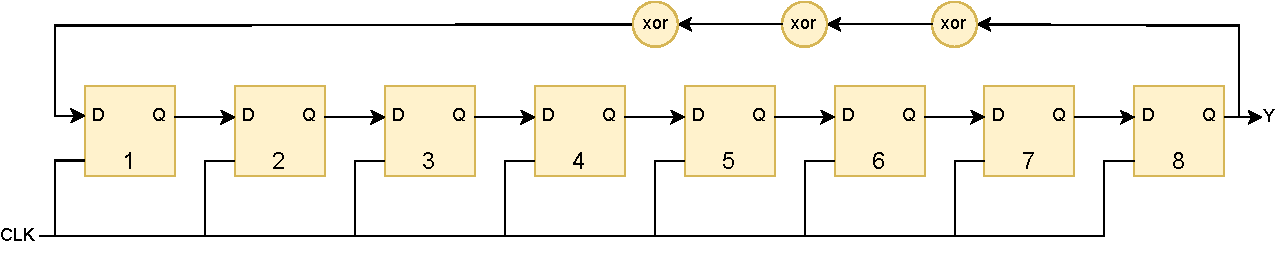
\includegraphics[width=1\linewidth]{pics/lfsr.pdf}
		\captionof{figure}[lfsr]{Abbildung eines Fibonacci-LFSR, angelehnt an \cite{}}
		\label{fig:lfsr}
	\end{minipage}

	\vspace{1em}
	Test so gehts weiter
	
	\subsection{Hardware Timer}
	% Nicht Konzept und umsetzung, sondern Register-Transfer-Ebene, Gatter-Ebene, Verdrahtung+Platzierung
	%Implementierung + Validierung
	\section{Schaltkreis Entwurf} %
	\subsection{Das Reaktionsspiel}
	\subsection{Register-Transfer-Ebene} %Hardwarebeschreibungssprache, Zustandsdiagramm und Vhdl code
	\subsection{Gatter-Ebene, Verdrahtung und Platzierung}
	
	\section{Umsetzung}
	\subsection{Implementierung}
	%Wokwi/Vhdl programm vorstellen
	\
	
	\section{Bewertung}
	\subsection{Zieleinhaltung}
	\subsection{Interpretation der Ergebnisse}
	
	\section{Zusammenfassung und Ausblick}
	
	
	% ----------------------------------------------------------------------------------------------------------
	% Abk�rzungsverzeichnis
	% ----------------------------------------------------------------------------------------------------------
	\section{Abk�rzungsverzeichnis}
	\rhead{Abk�rzungsverzeichnis}
	\vspace{1em}
	\begin{acronym}[KDE]
		\acro{IC}[IC]{integrierter Schaltkreis}
		\acrodefplural{IC}[IC]{integrierten Schaltkreises}
		\acro{LFSR}[LFSR]{linear r�ckgekoppeltes Schieberegister}
	\end{acronym}
	\pagebreak
	
		% ----------------------------------------------------------------------------------------------------------
	% Literatur
	% ----------------------------------------------------------------------------------------------------------
	%	\renewcommand\refname{Referenzen}
	%	\lhead{}
	%	\bibliographystyle{ieeetr}
	%	\bibliography{referenzen}
	%	\pagebreak
	
	\section{Literaturverzeichnis}
	\printbibliography
%	\rhead{Literaturverzeichnis}
%	\bibliographystyle{alpha}
%%	\bibliographystyle{ieeetr}
%	\renewcommand\refname{}
%	\bibliography{literatur}
	\pagebreak
	
	
	
\end{document}
